\documentclass[10pt,a4paper]{article}
\usepackage[margin=0.76in]{geometry}
\usepackage[T1]{fontenc}
\usepackage[utf8]{inputenc}
\usepackage{mathptmx,amsmath,booktabs,longtable,array,graphicx,xurl,hyperref,caption,float,needspace}
\usepackage{parskip}
\hypersetup{colorlinks=true,linkcolor=black,urlcolor=blue,pdftitle={Supplementary Information: Evaluating adaptive graph fusion},pdfauthor={Xinchen Geng}}
\captionsetup{font=small,labelfont=bf,justification=raggedright,singlelinecheck=false}
\renewcommand{\thetable}{S\arabic{table}}
\renewcommand{\thefigure}{S\arabic{figure}}
\renewcommand{\thesection}{S\arabic{section}}
\renewcommand{\thesubsection}{\thesection.\arabic{subsection}}
\setlength{\LTpre}{5pt}\setlength{\LTpost}{8pt}
\setlength{\parindent}{0pt}
\setlength{\parskip}{5pt}
\setlength{\emergencystretch}{2em}
\graphicspath{{figures/}}
\title{\textbf{Supplementary Information}\\[0.5em]\large Evaluating adaptive graph fusion for short-range weather forecasting with conditional local convolution}
\author{Xinchen Geng\\\small University of Southern California, Los Angeles, CA 90089, USA\\\small Correspondence: \texttt{gengx@usc.edu}}
\date{8 October 2026}
\begin{document}
\maketitle
\section{Scope, model inventory and evidence authority}
This supplement documents 46 newly trained models: 40 primary models (four tasks, two variants, five seeds) and six additional mean-fusion ablations (two tasks, three seeds). Every model completed 100 epochs in FP32 with zero-inclusive training, validation selection and test scoring. All reported accuracy values originate from the new-training evidence package. Historical checkpoint rescoring, screening trials and previous zero-exclusive results do not supply values to these tables.

The Conditional Local Convolution Recurrent Network (CLCRN) and Conditional Local Convolution (CLConv) were introduced by Lin et al.\cite{lin2022conditional}. The present contribution is an incremental adaptive graph-fusion (AGF) input extension and a controlled evaluation. The control is a matched local implementation: both variants use trainable node embeddings, whereas the upstream reference implementation registers those embeddings as a fixed buffer. The experiment therefore does not reproduce every upstream implementation choice.

The 40 primary replicates use seeds 2021--2025. The mean-fusion models use seeds 2023--2025 for temperature and humidity; the other 12 ablation entries reuse the corresponding control and AGF primary models. Thus the 18 ablation entries represent 18 selected models, of which only six are additional to the 40 primary models. The complete 46-row inventory, selected epochs, validation MAE, test scores, parameter counts, relative checkpoint paths and full SHA256 hashes are supplied in \path{data/model_inventory_46.csv}.

\section{Data, preprocessing and training protocol}
The four WeatherBench-derived tasks are 2-m temperature, relative humidity, joint 10-m wind components ($u,v$), and total cloud cover. Hourly 2010--2018 fields occupy a regular $32\times64$ latitude--longitude grid (2,048 nodes). Each example has 12 input hours and 12 target hours. Window starts are separated by 24 hours, and the chronological, unshuffled split contains 2,300 training, 329 validation and 657 test examples. There is one fixed split; training seeds are not cross-validation folds.

Normalization moments are computed from the original training-input arrays, separately for each physical variable and each wind component. Both inputs and targets are cast to float32 before in-place subtraction and division by these moments. This ordering is frozen as \path{curated_float32_then_train_only_standardization_v1}. Validation and test data use training moments. Predictions and targets are inverse-transformed to physical units before scoring.

\begin{table}[H]\centering\small\setlength{\tabcolsep}{5pt}\setlength{\parskip}{0pt}

\caption{Fixed protocol shared by every primary and ablation run.}\label{tab:protocol}

\begin{tabular}{p{0.37\linewidth}p{0.56\linewidth}}

\toprule
Item & Specification \\
\midrule

Training budget & 100 epochs; early stopping disabled \\

Optimizer & Adam; learning rate 0.01; $\epsilon=0.001$ \\

Batch size & 32 for training, validation and testing \\

Schedule & MultiStepLR at epochs 10, 20, 30, 40, 50; factor 0.95 \\

Gradient clipping & Global gradient norm 5 \\

Recurrent backbone & Two layers; 32 hidden units; one CLConv view \\

Geographic neighbours & 25 \\

Feature and backbone node embeddings & 8 dimensions each \\

AGF node embedding / output width & 10 / 8 dimensions \\

AGF retained neighbours & Top 4 per directed adjacency row \\

Decoder curriculum & Decay parameter 2,000 \\

Additional context & No calendar features or periodic encoding \\

Precision & FP32; AMP and TF32 disabled \\

Checkpoint selection & Earliest minimum full-validation zero-inclusive MAE \\

Runtime recorded in training manifest & Python 3.13.7; PyTorch 2.10.0+cu128 \\

GPU recorded in training manifest & NVIDIA GeForce RTX 5090 Laptop GPU; driver 610.88 \\

\bottomrule\end{tabular}\end{table}

\begin{table}[H]\centering\small\setlength{\tabcolsep}{5pt}\setlength{\parskip}{0pt}

\caption{Training-input normalization moments recorded by the evaluator. Physical units apply to both mean and standard deviation.}\label{tab:scalers}

\begin{tabular}{llrrl}

\toprule
Variable & Unit & Mean & Std. dev. & Raw dtype \\
\midrule

Temperature & K & 278.69592285 & 21.08552551 & float32 \\

Relative humidity & percentage points & 78.13786316 & 18.10952377 & float32 \\

Surface wind ($u$) & m\,s$^{-1}$ & -0.11169575 & 5.61085892 & float32 \\

Surface wind ($v$) & m\,s$^{-1}$ & 0.22041868 & 4.80938816 & float32 \\

Cloud cover & fraction & 0.67634958 & 0.36162654 & float32 \\

\bottomrule\end{tabular}\end{table}

Training and validation MAE include all finite targets, including valid zeros and negative values. A nonfinite prediction at a valid target raises an error. The new inference pass also rejects nonfinite error arrays instead of silently reducing the evaluation support. MAPE is not a primary metric. The raw target-zero audit is shown below; these zeros are observed values, not evidence of missing observations.

\begin{table}[H]\centering\small\setlength{\tabcolsep}{5pt}\setlength{\parskip}{0pt}

\caption{Exactly zero raw targets by split. Wind combines its two output components.}\label{tab:zeros}

\begin{tabular}{llrrr}

\toprule
Task & Split & Zero count & Total targets & Zero fraction (\%) \\
\midrule

Temperature & Train & 0 & 56,524,800 & 0.00000 \\

Temperature & Validation & 0 & 8,085,504 & 0.00000 \\

Temperature & Test & 0 & 16,146,432 & 0.00000 \\

Humidity & Train & 0 & 56,524,800 & 0.00000 \\

Humidity & Validation & 0 & 8,085,504 & 0.00000 \\

Humidity & Test & 0 & 16,146,432 & 0.00000 \\

Wind & Train & 0 & 113,049,600 & 0.00000 \\

Wind & Validation & 0 & 16,171,008 & 0.00000 \\

Wind & Test & 0 & 32,292,864 & 0.00000 \\

Cloud cover & Train & 2,234,618 & 56,524,800 & 3.95334 \\

Cloud cover & Validation & 315,357 & 8,085,504 & 3.90028 \\

Cloud cover & Test & 626,840 & 16,146,432 & 3.88222 \\

\bottomrule\end{tabular}\end{table}

The cloud-cover training correction changes the optimization objective as well as model selection. Raw cloud zeros can acquire small floating-point residuals after standardization and inversion; zero-inclusive support is defined by finiteness and does not depend on exact inverse-transformed equality to zero. The absence of exact raw zeros in the other tasks does not remove the need for a consistent evaluator.

All trainable parameters are materialized before constructing the optimizer. The frozen training workflow audits optimizer membership and gradient coverage. Checkpoints include optimizer, scheduler and random-number-generator states for interrupted-run recovery. cuDNN deterministic mode is enabled and benchmarking is disabled; this does not establish bitwise equivalence across different hardware or software environments.

\section{Validation selection and individual model results}
The selected checkpoint is the first epoch achieving the minimum MAE over the complete validation split among epochs 1--100. Test values do not enter selection. All 46 recorded histories contain epochs 1--100 exactly once; the inventory was checked against their earliest minima and against checkpoint/configuration/history SHA256 hashes. The following tables show the selected checkpoint and its cumulative 12-hour test scores. Validation MAE and test errors use the physical units indicated in each caption. Five seed labels do not imply paired stochastic streams across architectures.

\begin{table}[H]\centering\small\setlength{\tabcolsep}{5pt}\setlength{\parskip}{0pt}

\caption{Temperature primary models (K). Every model trained for 100 epochs.}\label{tab:seeds_temperature}

\begin{tabular}{llrrrr}

\toprule
Variant & Seed & Selected epoch & Validation MAE & Test MAE & Test RMSE \\
\midrule

Control & 2021 & 90 & 1.2411 & 1.2543 & 2.0440 \\

Control & 2022 & 80 & 1.3251 & 1.3380 & 2.1234 \\

Control & 2023 & 92 & 1.1584 & 1.1691 & 2.0634 \\

Control & 2024 & 66 & 1.2534 & 1.2722 & 2.1440 \\

Control & 2025 & 92 & 1.2576 & 1.2563 & 2.1314 \\

AGF & 2021 & 67 & 1.3028 & 1.3252 & 2.2316 \\

AGF & 2022 & 100 & 1.3533 & 1.3797 & 2.1862 \\

AGF & 2023 & 87 & 1.2724 & 1.2862 & 2.0017 \\

AGF & 2024 & 78 & 1.1045 & 1.1091 & 1.9559 \\

AGF & 2025 & 90 & 1.3439 & 1.3548 & 2.2149 \\

\bottomrule\end{tabular}\end{table}

\begin{table}[H]\centering\small\setlength{\tabcolsep}{5pt}\setlength{\parskip}{0pt}

\caption{Relative humidity primary models (percentage points). Every model trained for 100 epochs.}\label{tab:seeds_humidity}

\begin{tabular}{llrrrr}

\toprule
Variant & Seed & Selected epoch & Validation MAE & Test MAE & Test RMSE \\
\midrule

Control & 2021 & 100 & 4.5983 & 4.6677 & 7.2808 \\

Control & 2022 & 89 & 4.6034 & 4.6638 & 7.2816 \\

Control & 2023 & 82 & 4.5761 & 4.6394 & 7.1854 \\

Control & 2024 & 85 & 4.5756 & 4.6426 & 7.2712 \\

Control & 2025 & 66 & 4.5664 & 4.6263 & 7.2232 \\

AGF & 2021 & 97 & 4.4640 & 4.5222 & 6.9809 \\

AGF & 2022 & 85 & 4.4390 & 4.4986 & 6.9468 \\

AGF & 2023 & 78 & 4.4750 & 4.5348 & 7.0764 \\

AGF & 2024 & 87 & 4.4650 & 4.5279 & 6.9864 \\

AGF & 2025 & 94 & 4.5336 & 4.6024 & 7.0580 \\

\bottomrule\end{tabular}\end{table}

\begin{table}[H]\centering\small\setlength{\tabcolsep}{5pt}\setlength{\parskip}{0pt}

\caption{Surface wind primary models (m\,s$^{-1}$). Every model trained for 100 epochs.}\label{tab:seeds_component_of_wind}

\begin{tabular}{llrrrr}

\toprule
Variant & Seed & Selected epoch & Validation MAE & Test MAE & Test RMSE \\
\midrule

Control & 2021 & 78 & 1.2470 & 1.2441 & 1.9872 \\

Control & 2022 & 93 & 1.2382 & 1.2357 & 1.9607 \\

Control & 2023 & 98 & 1.2289 & 1.2258 & 1.9365 \\

Control & 2024 & 84 & 1.2547 & 1.2533 & 1.9908 \\

Control & 2025 & 89 & 1.2557 & 1.2512 & 1.9863 \\

AGF & 2021 & 86 & 1.2436 & 1.2392 & 1.9674 \\

AGF & 2022 & 82 & 1.2571 & 1.2548 & 2.0004 \\

AGF & 2023 & 98 & 1.2351 & 1.2334 & 1.9667 \\

AGF & 2024 & 84 & 1.2327 & 1.2309 & 1.9629 \\

AGF & 2025 & 94 & 1.3165 & 1.3201 & 2.1803 \\

\bottomrule\end{tabular}\end{table}

\begin{table}[H]\centering\small\setlength{\tabcolsep}{5pt}\setlength{\parskip}{0pt}

\caption{Cloud cover primary models (fraction). Every model trained for 100 epochs.}\label{tab:seeds_cloud_cover}

\begin{tabular}{llrrrr}

\toprule
Variant & Seed & Selected epoch & Validation MAE & Test MAE & Test RMSE \\
\midrule

Control & 2021 & 100 & 0.1472 & 0.1467 & 0.2494 \\

Control & 2022 & 99 & 0.1465 & 0.1458 & 0.2476 \\

Control & 2023 & 91 & 0.1501 & 0.1496 & 0.2523 \\

Control & 2024 & 91 & 0.1503 & 0.1496 & 0.2505 \\

Control & 2025 & 88 & 0.1485 & 0.1479 & 0.2501 \\

AGF & 2021 & 92 & 0.1475 & 0.1469 & 0.2499 \\

AGF & 2022 & 99 & 0.1494 & 0.1488 & 0.2508 \\

AGF & 2023 & 74 & 0.1472 & 0.1466 & 0.2440 \\

AGF & 2024 & 84 & 0.1485 & 0.1480 & 0.2507 \\

AGF & 2025 & 88 & 0.1521 & 0.1515 & 0.2495 \\

\bottomrule\end{tabular}\end{table}

\begin{table}[H]\centering\small\setlength{\tabcolsep}{5pt}\setlength{\parskip}{0pt}

\caption{Six additional mean-fusion models; temperature is in K and humidity in percentage points.}\label{tab:mean_models}

\begin{tabular}{llrrrr}

\toprule
Task & Seed & Selected epoch & Validation MAE & Test MAE & Test RMSE \\
\midrule

Temperature & 2023 & 89 & 1.2360 & 1.2544 & 1.9302 \\

Temperature & 2024 & 52 & 1.2059 & 1.2089 & 2.1240 \\

Temperature & 2025 & 98 & 1.3268 & 1.3382 & 2.0860 \\

Humidity & 2023 & 84 & 4.5342 & 4.5981 & 7.1015 \\

Humidity & 2024 & 93 & 4.5124 & 4.5763 & 7.0913 \\

Humidity & 2025 & 84 & 4.5603 & 4.6234 & 7.2037 \\

\bottomrule\end{tabular}\end{table}

\section{Primary statistics and exact-permutation sensitivity}
Primary MAE and RMSE pool errors over all 657 test examples, 12 leads, 2,048 nodes and output components. With $e_a=\widehat y_a-y_a$, $M$ is the total number of scalar targets:
\[
\mathrm{MAE}=M^{-1}\sum_{a=1}^{M}|e_a|,\qquad
\mathrm{RMSE}=\sqrt{M^{-1}\sum_{a=1}^{M}e_a^2}.
\]
Aggregation uses double precision on differences formed from inverse-transformed FP32 tensors. RMSE is obtained from the pooled squared errors, not an average of per-window or per-lead RMSEs. The scalar tasks have 16,146,432 targets per model; wind has 32,292,864.

For each task/metric, the unit of statistical analysis is a trained model. I report group means and sample standard deviations ($n=5$ per group), the difference $\Delta=\overline{x}_{\mathrm{AGF}}-\overline{x}_{\mathrm{control}}$, and the unadjusted two-sided 95\% Welch interval. With $v_g=s_g^2/n_g$, the standard error is $\sqrt{v_A+v_C}$ and the Welch--Satterthwaite degrees of freedom are
\[
\nu=\frac{(v_A+v_C)^2}{v_A^2/(n_A-1)+v_C^2/(n_C-1)}.
\]
The interval is $\Delta\pm t_{0.975,\nu}\sqrt{v_A+v_C}$. Two-sided Welch $p$ values receive Benjamini--Hochberg (BH) correction over all eight task/metric tests. Intervals are pointwise, not simultaneous confidence intervals.

\begin{table}[H]\centering\small\setlength{\tabcolsep}{5pt}\setlength{\parskip}{0pt}

\caption{Primary unweighted estimates. Errors retain task-specific physical units; differences are AGF minus control.}\label{tab:primary_estimates}

\begin{tabular}{llrrr}

\toprule
Task & Metric & Control (mean $\pm s$) & AGF (mean $\pm s$) & $\Delta$ [95\% CI] \\
\midrule

Temperature & MAE & $1.2580 \pm 0.0603$ & $1.2910 \pm 0.1075$ & $+0.0330$ $[-0.1004, +0.1664]$ \\

Temperature & RMSE & $2.1012 \pm 0.0445$ & $2.1181 \pm 0.1292$ & $+0.0168$ $[-0.1408, +0.1745]$ \\

Humidity & MAE & $4.6480 \pm 0.0174$ & $4.5372 \pm 0.0389$ & $-0.1108$ $[-0.1584, -0.0632]$ \\

Humidity & RMSE & $7.2484 \pm 0.0427$ & $7.0097 \pm 0.0550$ & $-0.2387$ $[-0.3113, -0.1661]$ \\

Wind & MAE & $1.2420 \pm 0.0114$ & $1.2557 \pm 0.0372$ & $+0.0137$ $[-0.0318, +0.0591]$ \\

Wind & RMSE & $1.9723 \pm 0.0234$ & $2.0155 \pm 0.0933$ & $+0.0432$ $[-0.0711, +0.1576]$ \\

Cloud cover & MAE & $0.1479 \pm 0.0017$ & $0.1484 \pm 0.0020$ & $+0.0005$ $[-0.0022, +0.0031]$ \\

Cloud cover & RMSE & $0.2500 \pm 0.0017$ & $0.2490 \pm 0.0028$ & $-0.0010$ $[-0.0045, +0.0025]$ \\

\bottomrule\end{tabular}\end{table}

The exact-permutation sensitivity uses the absolute difference in group means and enumerates all $\binom{10}{5}=252$ allocations, including the observed allocation. Its two-sided $p$ value is the fraction at least as extreme as observed (with $10^{-12}$ numerical comparison tolerance). Exactness holds under exchangeable group labels, not the weaker equal-means null with arbitrary unequal variances. Its eight $p$ values form a separate BH family; this sensitivity does not replace primary Welch inference. No paired sign test is used.

\begin{table}[H]\centering\small\setlength{\tabcolsep}{5pt}\setlength{\parskip}{0pt}

\caption{Primary significance and permutation sensitivity; each pair of $q$ columns uses its own eight-comparison family.}\label{tab:primary_tests}

\begin{tabular}{llrrrrr}

\toprule
Task & Metric & Change (\%) & Welch $p$ & Welch $q$ & Exact $p$ & Exact $q$ \\
\midrule

Temperature & MAE & +2.625 & 0.570054 & 0.760072 & 0.555556 & 0.770975 \\

Temperature & RMSE & +0.800 & 0.794234 & 0.794234 & 0.777778 & 0.777778 \\

Humidity & MAE & -2.384 & 0.001510 & 0.006040 & 0.007937 & 0.031746 \\

Humidity & RMSE & -3.294 & 0.000082 & 0.000653 & 0.007937 & 0.031746 \\

Wind & MAE & +1.100 & 0.469944 & 0.760072 & 0.634921 & 0.770975 \\

Wind & RMSE & +2.193 & 0.365690 & 0.760072 & 0.452381 & 0.770975 \\

Cloud cover & MAE & +0.306 & 0.707722 & 0.794234 & 0.674603 & 0.770975 \\

Cloud cover & RMSE & -0.408 & 0.510257 & 0.760072 & 0.619048 & 0.770975 \\

\bottomrule\end{tabular}\end{table}

Only humidity MAE and RMSE satisfy $q<0.05$ in both families. Their mean reductions are 2.38\% and 3.29\%, respectively. For both humidity metrics the permutation $p$ is $2/252=0.007937$ and the separately corrected $q$ is 0.031746. The other six comparisons do not establish differences at the stated threshold. Failure to reject a null is not proof of equal performance. These tests quantify training-seed variation on the fixed split and do not estimate variation across climates, periods, splits or datasets.

\section{Latitude-weighted sensitivity}
For latitude $\phi_i$, I replace unit weights by $w_i=\cos\phi_i$ and calculate
\[
\mathrm{MAE}_w=\frac{\sum_a w_a|e_a|}{\sum_a w_a},\qquad
\mathrm{RMSE}_w=\sqrt{\frac{\sum_a w_a e_a^2}{\sum_a w_a}}.
\]
The evaluator normalizes node weights to mean one; repeating them over windows, leads and channels is algebraically equivalent to the displayed denominator. This changes evaluation only, not training, validation selection or checkpoints. Its eight Welch tests constitute a separate sensitivity family. Humidity remains the only task with both corrected metrics below 0.05.

\begin{table}[H]\centering\small\setlength{\tabcolsep}{5pt}\setlength{\parskip}{0pt}

\caption{Latitude-weighted scores, pointwise Welch intervals and separately corrected $q$ values.}\label{tab:weighted}

\begin{tabular}{llrrrr}

\toprule
Task & Metric & Control mean & AGF mean & $\Delta$ [95\% CI] & BH $q$ \\
\midrule

Temperature & MAE & 1.1722 & 1.2383 & $+0.0661$ $[-0.0971, +0.2293]$ & 0.659747 \\

Temperature & RMSE & 2.0135 & 2.0503 & $+0.0369$ $[-0.1136, +0.1873]$ & 0.659747 \\

Humidity & MAE & 4.6573 & 4.5300 & $-0.1273$ $[-0.1910, -0.0637]$ & 0.010764 \\

Humidity & RMSE & 7.2278 & 6.9485 & $-0.2793$ $[-0.3689, -0.1896]$ & 0.000871 \\

Wind & MAE & 1.2191 & 1.2312 & $+0.0121$ $[-0.0331, +0.0572]$ & 0.659747 \\

Wind & RMSE & 1.9173 & 1.9585 & $+0.0412$ $[-0.0729, +0.1553]$ & 0.659747 \\

Cloud cover & MAE & 0.1595 & 0.1600 & $+0.0005$ $[-0.0024, +0.0034]$ & 0.692620 \\

Cloud cover & RMSE & 0.2528 & 0.2518 & $-0.0009$ $[-0.0044, +0.0025]$ & 0.659747 \\

\bottomrule\end{tabular}\end{table}

\section{Persistence on the same split}
Persistence repeats the final observed input over all 12 forecast leads. It is evaluated once, with the same inverse transformation, test split, zero-inclusive target support and unweighted aggregation as the trained models. It has no training-seed standard deviation. Control and AGF entries below are means of their five trained replicates. The table is descriptive; persistence is not an additional primary hypothesis test. Historical published CLCRN scores have different evaluation provenance and are not included in this matched table.

\begin{table}[H]\centering\small\setlength{\tabcolsep}{5pt}\setlength{\parskip}{0pt}

\caption{Current-split cumulative 12-hour error. Humidity units are percentage points; cloud cover is a fraction.}\label{tab:context}

\begin{tabular}{llrrr}

\toprule
Task & Method & Training replicates & MAE & RMSE \\
\midrule

Temperature & Persistence & -- & 1.4214 & 2.7001 \\

Temperature & Control & 5 & 1.2580 & 2.1012 \\

Temperature & CLCRN-AGF & 5 & 1.2910 & 2.1181 \\

Humidity & Persistence & -- & 6.4248 & 10.4471 \\

Humidity & Control & 5 & 4.6480 & 7.2484 \\

Humidity & CLCRN-AGF & 5 & 4.5372 & 7.0097 \\

Wind & Persistence & -- & 1.5372 & 2.5354 \\

Wind & Control & 5 & 1.2420 & 1.9723 \\

Wind & CLCRN-AGF & 5 & 1.2557 & 2.0155 \\

Cloud cover & Persistence & -- & 0.1620 & 0.2725 \\

Cloud cover & Control & 5 & 0.1479 & 0.2500 \\

Cloud cover & CLCRN-AGF & 5 & 0.1484 & 0.2490 \\

\bottomrule\end{tabular}\end{table}

\section{Three-seed component ablation}
The no-AGF condition removes the complete input augmentation and is exactly the matched control. Mean fusion retains the two AGF projections but uses $\mathbf z=(\mathbf q+\mathbf r)/2$ instead of the learned gate. Full AGF uses $\mathbf z=\mathbf g\odot\mathbf q+(1-\mathbf g)\odot\mathbf r$. Both branches use the same pre-CLConv input: $\mathbf q$ is graph-aggregated and $\mathbf r$ is a node-wise residual linear projection. Neither branch is a CLConv output. All conditions receive the same 100-epoch FP32 budget, and every row uses seeds 2023--2025.

\begin{table}[H]\centering\small\setlength{\tabcolsep}{5pt}\setlength{\parskip}{0pt}

\caption{Aligned three-seed ablation. Values are mean $\pm$ sample standard deviation, not five-seed summaries.}\label{tab:ablation}

\begin{tabular}{llrr}

\toprule
Task & Variant & MAE & RMSE \\
\midrule

Temperature & No AGF (control) & $1.2325 \pm 0.0555$ & $2.1129 \pm 0.0433$ \\

Temperature & Mean fusion & $1.2672 \pm 0.0656$ & $2.0468 \pm 0.1027$ \\

Temperature & Full AGF & $1.2500 \pm 0.1268$ & $2.0575 \pm 0.1382$ \\

Humidity & No AGF (control) & $4.6361 \pm 0.0086$ & $7.2266 \pm 0.0430$ \\

Humidity & Mean fusion & $4.5993 \pm 0.0236$ & $7.1322 \pm 0.0622$ \\

Humidity & Full AGF & $4.5550 \pm 0.0412$ & $7.0403 \pm 0.0475$ \\

\bottomrule\end{tabular}\end{table}

Humidity has progressively lower mean errors from control to mean fusion to learned gating in this subset. Temperature is metric-dependent: control has the lowest mean MAE, while mean fusion has the lowest mean RMSE. The three-seed ablation is descriptive and does not establish that gating is universally necessary. Individual control/AGF values are reported above; the six additional models appear in Table~\ref{tab:mean_models}. The complete 18-row aligned file is \path{data/ablation_per_seed.csv}.

\section{Missing-input diagnostic: 64 windows and three masks}
The diagnostic uses 64 deterministic, approximately equally spaced test indices spanning the 657-window chronology, including indices 0 and 656. The exact indices are recorded separately for each task. All primary models share this subset and mask seeds 11, 22 and 33. For each test example and nonzero nominal ratio $r\in\{0.1,0.2,0.3,0.4\}$, the evaluator samples $\lfloor2048r\rfloor$ nodes without replacement. The example's mask is held fixed over all 12 input hours and all input channels. Different examples receive different draws. For a given ratio/mask seed, the same masks are reused across architectures and training seeds.

Masked standardized inputs are set to zero, corresponding to the training mean in physical units. This is input replacement, not target masking, and is distinct from the valid zero-target protocol. Training is unchanged. At each ratio, three relative MAE increases are averaged within each trained seed; the displayed mean and sample standard deviation are then computed across the five trained seeds. Masks are nested technical repeats, not 15 independent training replicates. Each relative increase uses the same checkpoint's clean MAE on the same 64-window subset:
\[
100\,\frac{\mathrm{MAE}_{\mathrm{masked},s,m}-\mathrm{MAE}_{\mathrm{clean},s}}{\mathrm{MAE}_{\mathrm{clean},s}}.
\]

\begin{table}[H]\centering\small\setlength{\tabcolsep}{5pt}\setlength{\parskip}{0pt}

\caption{Relative MAE increase (\%) on the shared 64-window subset. At zero missingness every relative increase is zero by definition.}\label{tab:missing}

\begin{tabular}{lrrrr}

\toprule
Task & Nominal ratio & Masked nodes & Control (mean $\pm s$) & AGF (mean $\pm s$) \\
\midrule

Temperature & 0.1 & 204 & $115.80 \pm 5.96$ & $114.32 \pm 12.85$ \\

Temperature & 0.2 & 409 & $233.37 \pm 11.93$ & $229.99 \pm 25.54$ \\

Temperature & 0.3 & 614 & $352.13 \pm 17.85$ & $346.55 \pm 38.11$ \\

Temperature & 0.4 & 819 & $474.09 \pm 23.92$ & $465.95 \pm 50.67$ \\

Humidity & 0.1 & 204 & $17.79 \pm 0.31$ & $18.01 \pm 0.30$ \\

Humidity & 0.2 & 409 & $35.87 \pm 0.58$ & $36.42 \pm 0.61$ \\

Humidity & 0.3 & 614 & $54.12 \pm 0.82$ & $55.18 \pm 0.89$ \\

Humidity & 0.4 & 819 & $72.99 \pm 1.02$ & $74.71 \pm 1.19$ \\

Wind & 0.1 & 204 & $20.29 \pm 0.64$ & $20.12 \pm 0.22$ \\

Wind & 0.2 & 409 & $41.47 \pm 1.12$ & $41.03 \pm 0.70$ \\

Wind & 0.3 & 614 & $63.44 \pm 1.57$ & $62.73 \pm 1.39$ \\

Wind & 0.4 & 819 & $85.75 \pm 1.92$ & $84.67 \pm 2.28$ \\

Cloud cover & 0.1 & 204 & $7.50 \pm 0.41$ & $7.89 \pm 0.85$ \\

Cloud cover & 0.2 & 409 & $15.86 \pm 0.89$ & $16.67 \pm 1.50$ \\

Cloud cover & 0.3 & 614 & $25.05 \pm 1.48$ & $26.45 \pm 1.97$ \\

Cloud cover & 0.4 & 819 & $35.49 \pm 2.24$ & $37.52 \pm 2.29$ \\

\bottomrule\end{tabular}\end{table}

AGF does not show uniform missing-input robustness: relative increases are slightly lower for temperature and wind, but higher for humidity and cloud cover. Relative degradation is not a comparison of absolute masked errors between models with different clean errors. Absolute clean/masked MAE and RMSE for all 520 records are supplied in \path{data/robustness_per_seed_mask.csv}. This sampled input-replacement diagnostic is not a full-test benchmark or a test of actual missing-observation patterns, and no robustness significance claim is made.

\section{Full-test gate statistics}
The gate is $\mathbf g=\sigma(W_g[\mathbf r\Vert\mathbf q]+b_g)$ and its value weights the graph-aggregated branch in the fusion above. Statistics are collected from all scalar gate outputs before any channel averaging. Each AGF model contributes $657\times12\times2048\times8=129{,}171{,}456$ values; the five-model task pool has 645,857,280 values. All 100 histogram bins over $[0,1]$ sum to the corresponding scalar count. A value displayed as 1.0000 can result from floating-point sigmoid saturation or rounding; it does not indicate a hard selection mechanism.

\begin{table}[H]\centering\small\setlength{\tabcolsep}{5pt}\setlength{\parskip}{0pt}

\caption{Gate statistics for every AGF training seed. Standard deviation describes scalar gate dispersion within a model.}\label{tab:gate_seed}

\begin{tabular}{llrrrr}

\toprule
Task & Seed & Mean & Population SD & Minimum & Maximum \\
\midrule

Temperature & 2021 & 0.6156 & 0.2331 & 0.0014 & 0.9967 \\

Temperature & 2022 & 0.6230 & 0.2706 & 0.0010 & 1.0000 \\

Temperature & 2023 & 0.6260 & 0.1393 & 0.1331 & 0.9825 \\

Temperature & 2024 & 0.5789 & 0.1512 & 0.0427 & 0.9746 \\

Temperature & 2025 & 0.5573 & 0.1381 & 0.0640 & 0.9644 \\

Humidity & 2021 & 0.5853 & 0.2412 & 0.0018 & 0.9995 \\

Humidity & 2022 & 0.5685 & 0.2130 & 0.0088 & 0.9992 \\

Humidity & 2023 & 0.6644 & 0.2369 & 0.0164 & 0.9990 \\

Humidity & 2024 & 0.5236 & 0.2417 & 0.0018 & 0.9981 \\

Humidity & 2025 & 0.5107 & 0.2569 & 0.0014 & 0.9993 \\

Wind & 2021 & 0.4950 & 0.1133 & 0.0994 & 0.8989 \\

Wind & 2022 & 0.5045 & 0.1439 & 0.0705 & 0.9541 \\

Wind & 2023 & 0.5129 & 0.1210 & 0.0600 & 0.9177 \\

Wind & 2024 & 0.4954 & 0.1241 & 0.0845 & 0.9529 \\

Wind & 2025 & 0.5304 & 0.1427 & 0.0486 & 0.9418 \\

Cloud cover & 2021 & 0.4632 & 0.2173 & 0.0175 & 0.9850 \\

Cloud cover & 2022 & 0.4416 & 0.2180 & 0.0088 & 0.9970 \\

Cloud cover & 2023 & 0.5452 & 0.1870 & 0.0418 & 0.9799 \\

Cloud cover & 2024 & 0.4603 & 0.1958 & 0.0023 & 0.9763 \\

Cloud cover & 2025 & 0.4666 & 0.2044 & 0.0101 & 0.9702 \\

\bottomrule\end{tabular}\end{table}

\begin{table}[H]\centering\small\setlength{\tabcolsep}{5pt}\setlength{\parskip}{0pt}

\caption{Gate moments pooled across five AGF seeds, with equal scalar support per model.}\label{tab:gate_pool}

\begin{tabular}{lrrrr}

\toprule
Task & Mean & Pooled population SD & Minimum & Maximum \\
\midrule

Temperature & 0.6001 & 0.1963 & 0.0010 & 1.0000 \\

Humidity & 0.5705 & 0.2445 & 0.0014 & 0.9995 \\

Wind & 0.5076 & 0.1302 & 0.0486 & 0.9541 \\

Cloud cover & 0.4754 & 0.2080 & 0.0023 & 0.9970 \\

\bottomrule\end{tabular}\end{table}

The pooled variance includes both within-model dispersion and differences among seed means; it is not the standard deviation of five seed means. The gate values are correlated over space and time and are not independent inferential samples. Their magnitudes do not prove physical interpretability, causal importance or forecast improvement. Both projections have learned scales, so a numerical gate coefficient alone does not measure a branch's contribution to output error.

\section{Forecast-lead support and reproducibility boundaries}
Exact-lead scores use only lead $h$; cumulative scores pool leads 1 through $h$. They must not be interchanged. The machine-readable horizon file contains 480 rows ($40\times12$), each with both definitions. At lead 12, every cumulative value agrees with its primary aggregate. The table below illustrates exact-lead scores at 6 and 12 hours; all leads remain available in \path{data/horizon_per_seed.csv}. No additional per-lead significance family is claimed.

\begin{table}[H]\centering\small\setlength{\tabcolsep}{5pt}\setlength{\parskip}{0pt}

\caption{Exact-lead scores (mean $\pm$ sample SD over five models), in the task-specific physical units.}\label{tab:horizons}

\begin{tabular}{llrrr}

\toprule
Task & Variant & Lead (h) & Exact MAE & Exact RMSE \\
\midrule

Temperature & Control & 6 & $1.3388 \pm 0.0776$ & $2.1614 \pm 0.0615$ \\

Temperature & Control & 12 & $1.8639 \pm 0.1216$ & $2.8042 \pm 0.1336$ \\

Temperature & AGF & 6 & $1.3488 \pm 0.0931$ & $2.1260 \pm 0.0900$ \\

Temperature & AGF & 12 & $2.0530 \pm 0.2591$ & $2.9300 \pm 0.2845$ \\

Humidity & Control & 6 & $4.9726 \pm 0.0206$ & $7.3972 \pm 0.0539$ \\

Humidity & Control & 12 & $6.5617 \pm 0.0295$ & $9.2681 \pm 0.0595$ \\

Humidity & AGF & 6 & $4.7942 \pm 0.0387$ & $6.9943 \pm 0.0730$ \\

Humidity & AGF & 12 & $6.5154 \pm 0.0749$ & $9.2202 \pm 0.0819$ \\

Wind & Control & 6 & $1.2720 \pm 0.0095$ & $1.8948 \pm 0.0193$ \\

Wind & Control & 12 & $1.9213 \pm 0.0247$ & $2.7604 \pm 0.0395$ \\

Wind & AGF & 6 & $1.2857 \pm 0.0337$ & $1.9330 \pm 0.0749$ \\

Wind & AGF & 12 & $1.9446 \pm 0.0745$ & $2.8249 \pm 0.1559$ \\

Cloud cover & Control & 6 & $0.1555 \pm 0.0019$ & $0.2560 \pm 0.0019$ \\

Cloud cover & Control & 12 & $0.1927 \pm 0.0026$ & $0.3051 \pm 0.0020$ \\

Cloud cover & AGF & 6 & $0.1560 \pm 0.0021$ & $0.2550 \pm 0.0028$ \\

Cloud cover & AGF & 12 & $0.1933 \pm 0.0032$ & $0.3034 \pm 0.0046$ \\

\bottomrule\end{tabular}\end{table}

All 46 inference records were checked against their checkpoint, configuration, summary, training-history and run-manifest digests. The independent supplement audit recomputes means, sample standard deviations, Welch statistics and intervals, all 252 permutation allocations, BH corrections, nested robustness summaries and pooled gate moments. This audit validates the released records and calculations; it is not a new training experiment or an independent implementation of the network.

The maximum absolute difference between the new inference MAE/RMSE and the new training-summary metrics is $4.061\times10^{-10}$. Small differences arise from aggregation order; historical metrics are not used as the reference for this check.

The source snapshot and supplied processed arrays are the operational reproduction boundary. Data-source JSON files record the SHA256 hashes of \path{trn.pkl}, \path{val.pkl}, \path{test.pkl} and \path{position_info.pkl}, together with dimensions and scaler moments. This package does not establish a checksum-verified reconstruction from the original ERA5 archive, broader weather-model competitiveness, uncertainty under alternative data splits, or attribution to a particular physical process. Full retraining requires the processed input arrays, frozen training source, configurations and compatible accelerator environment. Re-running \path{build_supplement.py} rebuilds this supplement and its numerical audit from the recorded results; it does not rerun inference.

No fresh training-throughput, inference-latency or memory benchmark is introduced here. Analysis wall-clock fields include evaluation and diagnostics and are not matched timing measurements. Any historical efficiency measurements discussed in the main article retain their separate provenance and must not be presented as measurements of these 46 new checkpoints.

\section{Evidence files accompanying this supplement}
The accompanying \path{data/} directory contains the following inspectable records. Complete file digests and original source locations are listed in \path{supplement_sources.json}; the supplement's own audit results are in \path{supplement_validation.json}.
\begin{itemize}
\item \path{model_inventory_46.csv}: the complete new-model inventory with selected validation epochs and full checkpoint hashes.
\item \path{primary_per_seed.csv}, \path{table1_primary_statistics.csv}: 40 primary model values and eight unweighted comparisons, including Welch and exact-permutation statistics.
\item \path{latitude_weighted_sensitivity.csv}: separately corrected spatial-weighting sensitivity.
\item \path{ablation_per_seed.csv}, \path{table3_ablation_statistics.csv}: 18 aligned entries and six three-seed summaries.
\item \path{table2_current_context.csv}, \path{persistence_*.json}: same-split persistence and model context.
\item \path{raw_target_zero_fractions.csv}, \path{dataset_*.json}: raw-zero support, split dimensions, moments and input-file hashes.
\item \path{horizon_per_seed.csv}: 480 exact-lead/cumulative records.
\item \path{robustness_indices_*.json}, \path{robustness_per_seed_mask.csv}, \path{robustness_summary.csv}: exact 64-window subsets, 520 clean/masked records, and summaries respecting mask nesting.
\item \path{gate_per_seed.csv}, \path{gate_histogram.csv}, \path{table4_gate_statistics.csv}: 20 model-level records, 100-bin histograms and pooled full-test gate statistics.
\item \path{inference_*.json}: 46 new-checkpoint inference records, selected epochs, configuration/checkpoint/history hashes, metric sufficient sums and diagnostics where applicable.
\item \path{verification_report.json}, \path{provenance_manifest.json}, \path{analysis_code_manifest.json}: original completion/selection checks, source identities and frozen analysis-code provenance.
\end{itemize}

Full-resolution supplementary figures follow. Figure S1 is conceptual; Figures S2--S4 are generated from the same new evidence described above. They do not introduce additional trained models or statistical families.

\begin{thebibliography}{1}
\bibitem{lin2022conditional} Lin, H. et al. Conditional local convolution for spatio-temporal meteorological forecasting. \textit{Proc. AAAI Conf. Artif. Intell.} \textbf{36}, 7470--7478 (2022).
\end{thebibliography}

\clearpage\section{Supplementary figures}

\begin{figure}[H]
\centering
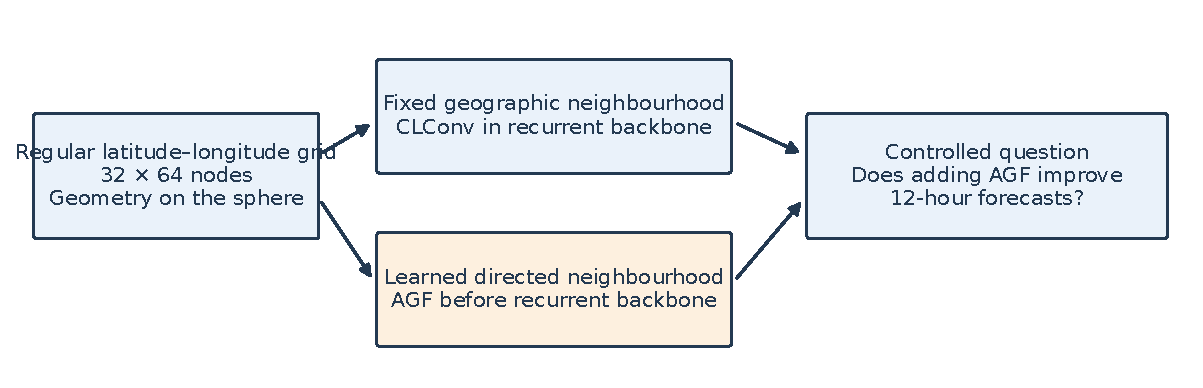
\includegraphics[width=0.96\linewidth,height=0.70\textheight,keepaspectratio]{fig1_motivation.pdf}
\caption{\textbf{Scope of the controlled comparison.} The fixed geographic
neighbourhood is used by CLConv in both models. CLCRN-AGF adds a learned
directed neighbourhood before the recurrent backbone. This conceptual
diagram makes no claim that either neighbourhood identifies a particular
physical process or that a measured form of geometric overfitting is reduced.}
\label{fig:background}
\end{figure}

\begin{figure}[H]
\centering
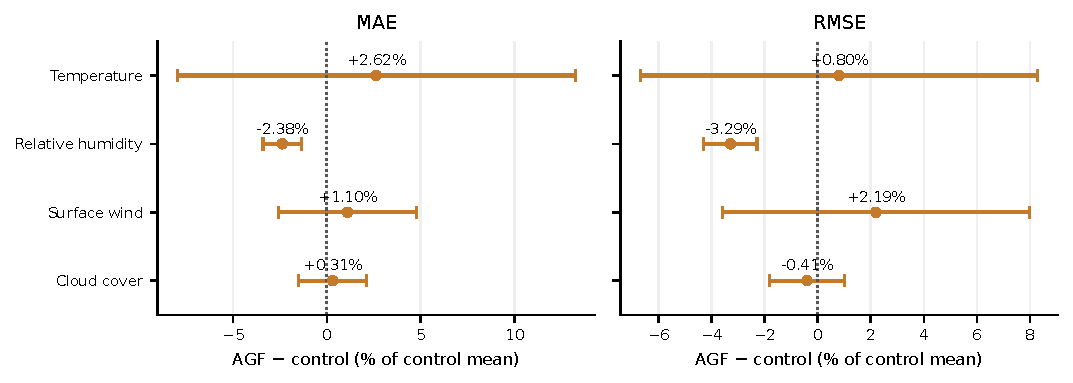
\includegraphics[width=0.96\linewidth,height=0.70\textheight,keepaspectratio]{fig6_primary_effects.pdf}
\caption{AGF-minus-control mean differences and 95\% Welch intervals from Table~\ref{tab:primary_estimates}, divided by the corresponding observed control mean and expressed as percentages. Negative values favour AGF. These are rescaled difference intervals, not confidence intervals from a separate ratio estimator. No single selected AGF run or historical schedule result enters this figure.}
\label{fig:decomp}
\end{figure}
\clearpage
\begin{figure}[H]
\centering
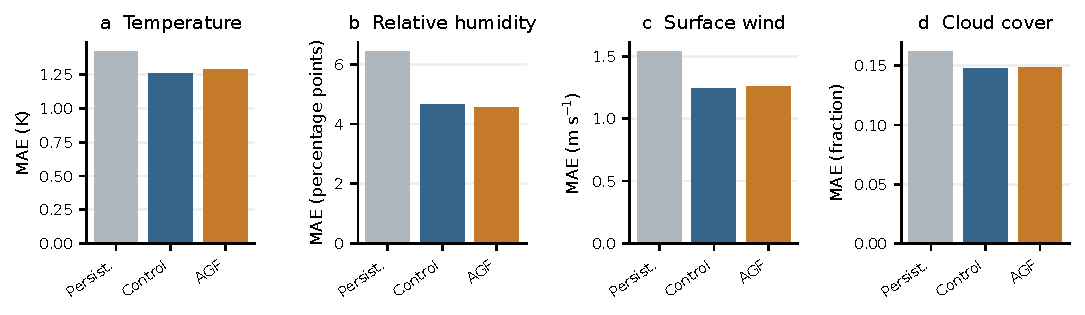
\includegraphics[width=0.96\linewidth,height=0.70\textheight,keepaspectratio]{fig3_context_current_split.pdf}
\caption{Current-split cumulative 12-hour MAE. Persistence is deterministic; control and AGF are five-seed means. All results use the same zero-inclusive, spatially unweighted evaluator. Panels have task-specific physical units. This is contextual, not a causal decomposition of schedule changes.}
\label{fig:context}
\end{figure}

\begin{figure}[H]
\centering
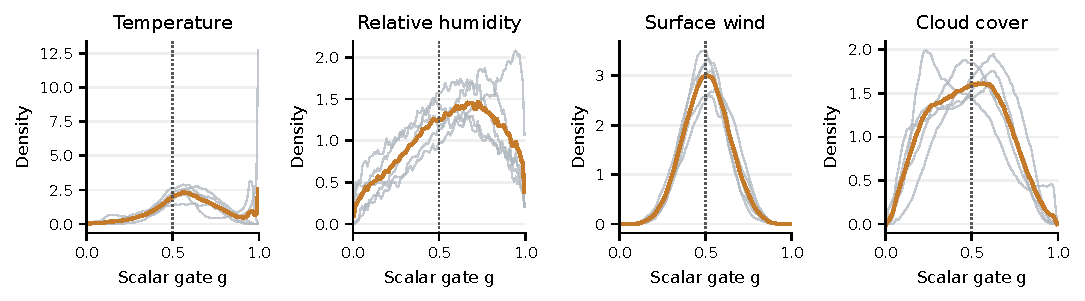
\includegraphics[width=0.96\linewidth,height=0.70\textheight,keepaspectratio]{fig8_gate_consistent.pdf}
\caption{Full-test distributions of scalar sigmoid gates for all four tasks and the same five AGF checkpoints as the primary model tables above. Gates are collected over 657 test windows, 12 input hours, 2048 nodes and 8 output channels per seed. Thin grey curves are individual seeds and the coloured curve is the pooled 100-bin density. The gate mixes adaptive graph aggregation and a nodewise residual projection before CLConv. Gate magnitudes do not by themselves measure the relative contribution of the two branches.}
\label{fig:gate}
\end{figure}

\end{document}
